\documentclass{standalone}
\usepackage{tikz}
\usetikzlibrary{patterns}
\usetikzlibrary{positioning}
\usetikzlibrary{patterns, positioning}
\usetikzlibrary{shapes.misc}
\usepackage[outline]{contour}
\contourlength{1.5pt} 


\begin{document}
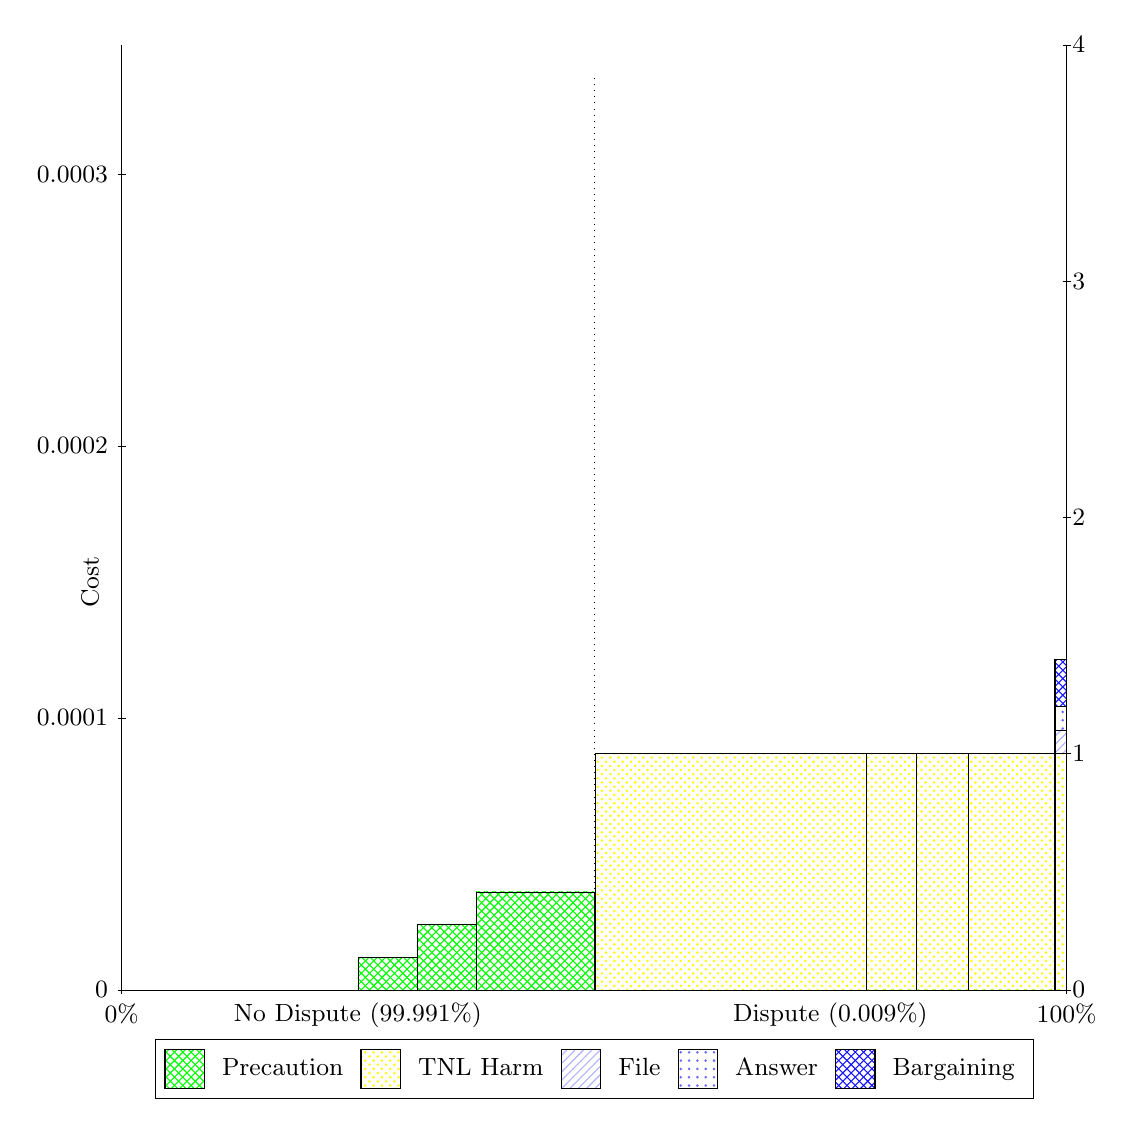
\begin{tikzpicture}
\draw[pattern=crosshatch, pattern color=green,draw=black,very thin] (4.5,2.5) rectangle (5.25,2.9144);
\draw[pattern=crosshatch, pattern color=green,draw=black,very thin] (5.25,2.5) rectangle (6,3.3289);
\draw[pattern=crosshatch, pattern color=green,draw=black,very thin] (6,2.5) rectangle (7.5,3.7433);
\draw[pattern=crosshatch, pattern color=green,draw=black,very thin] (7.5,2.5) rectangle (7.5154,2.5);
\draw[pattern=north east lines, pattern color=blue!30,draw=black,very thin] (7.5,2.5) rectangle (7.5154,2.8);
\draw[pattern=dots,  pattern color=blue!60,draw=black,very thin] (7.5,2.8) rectangle (7.5154,3.1);
\draw[pattern=crosshatch,      pattern color=blue!90,draw=black,very thin] (7.5,3.1) rectangle (7.5154,3.7);
\draw[pattern=crosshatch dots, pattern color=yellow,draw=black,very thin] (7.5154,2.5) rectangle (10.96,5.5);
\draw[pattern=crosshatch, pattern color=green,draw=black,very thin] (10.96,2.5) rectangle (11.593,2.5);
\draw[pattern=crosshatch dots, pattern color=yellow,draw=black,very thin] (10.96,2.5) rectangle (11.593,5.5);
\draw[pattern=crosshatch, pattern color=green,draw=black,very thin] (11.593,2.5) rectangle (12.252,2.5001);
\draw[pattern=crosshatch dots, pattern color=yellow,draw=black,very thin] (11.593,2.5001) rectangle (12.252,5.5001);
\draw[pattern=crosshatch, pattern color=green,draw=black,very thin] (12.252,2.5) rectangle (13.347,2.5001);
\draw[pattern=crosshatch dots, pattern color=yellow,draw=black,very thin] (12.252,2.5001) rectangle (13.347,5.5001);
\draw[pattern=crosshatch dots, pattern color=yellow,draw=black,very thin] (13.347,2.5) rectangle (13.357,5.5);
\draw[pattern=north east lines, pattern color=blue!30,draw=black,very thin] (13.347,5.5) rectangle (13.357,5.8);
\draw[pattern=dots,  pattern color=blue!60,draw=black,very thin] (13.347,5.8) rectangle (13.357,6.1);
\draw[pattern=crosshatch,      pattern color=blue!90,draw=black,very thin] (13.347,6.1) rectangle (13.357,6.7);
\draw[pattern=crosshatch, pattern color=green,draw=black,very thin] (13.357,2.5) rectangle (13.493,2.5);
\draw[pattern=crosshatch dots, pattern color=yellow,draw=black,very thin] (13.357,2.5) rectangle (13.493,5.5);
\draw[pattern=north east lines, pattern color=blue!30,draw=black,very thin] (13.357,5.5) rectangle (13.493,5.8);
\draw[pattern=dots,  pattern color=blue!60,draw=black,very thin] (13.357,5.8) rectangle (13.493,6.1);
\draw[pattern=crosshatch,      pattern color=blue!90,draw=black,very thin] (13.357,6.1) rectangle (13.493,6.7);
\draw[pattern=crosshatch, pattern color=green,draw=black,very thin] (13.493,2.5) rectangle (13.5,2.5001);
\draw[pattern=crosshatch dots, pattern color=yellow,draw=black,very thin] (13.493,2.5001) rectangle (13.5,5.5001);
\draw[pattern=north east lines, pattern color=blue!30,draw=black,very thin] (13.493,5.5001) rectangle (13.5,5.8001);
\draw[pattern=dots,  pattern color=blue!60,draw=black,very thin] (13.493,5.8001) rectangle (13.5,6.1001);
\draw[pattern=crosshatch,      pattern color=blue!90,draw=black,very thin] (13.493,6.1001) rectangle (13.5,6.7001);
\draw[black,very thin] (1.5,2.5) -- (1.5,14.5);
\node[font=\small,rotate=90,text=black, anchor=center] at (1.1, 7.6806) {Cost};
\draw[black,very thin] (1.45,2.5) -- (1.55,2.5);
\node[font=\small,text=black, anchor=east] at (1.45, 2.5) {0};
\draw[black,very thin] (1.45,5.9537) -- (1.55,5.9537);
\node[font=\small,text=black, anchor=east] at (1.45, 5.9537) {0.0001};
\draw[black,very thin] (1.45,9.4075) -- (1.55,9.4075);
\node[font=\small,text=black, anchor=east] at (1.45, 9.4075) {0.0002};
\draw[black,very thin] (1.45,12.861) -- (1.55,12.861);
\node[font=\small,text=black, anchor=east] at (1.45, 12.861) {0.0003};

\draw[black,dotted,very thin] (7.5,2.86) -- (7.5,14.14);
\draw[black,very thin] (13.5,2.5) -- (13.5,14.5);
\draw[black,very thin] (13.45,2.5) -- (13.55,2.5);
\node[font=\small,text=black, anchor=west] at (13.45, 2.5) {0};
\draw[black,very thin] (13.45,5.5) -- (13.55,5.5);
\node[font=\small,text=black, anchor=west] at (13.45, 5.5) {1};
\draw[black,very thin] (13.45,8.5) -- (13.55,8.5);
\node[font=\small,text=black, anchor=west] at (13.45, 8.5) {2};
\draw[black,very thin] (13.45,11.5) -- (13.55,11.5);
\node[font=\small,text=black, anchor=west] at (13.45, 11.5) {3};
\draw[black,very thin] (13.45,14.5) -- (13.55,14.5);
\node[font=\small,text=black, anchor=west] at (13.45, 14.5) {4};

\draw[black,very thin] (1.5,2.5) -- (13.5,2.5);
\draw[black,very thin] (1.5,2.45) -- (1.5,2.55);
\node[font=\small,text=black, anchor=north] at (1.5, 2.45) {0\%};
\draw[black,very thin] (13.5,2.45) -- (13.5,2.55);
\node[font=\small,text=black, anchor=north] at (13.5, 2.45) {100\%};

\node[font=\small,text=black,anchor=south] at (4.5, 1.9) {No\ Dispute\ (99.991\%)};
\node[font=\small,text=black,anchor=south] at (10.5, 1.9) {Dispute\ (0.009\%)};
\draw (7.5,2.5) node (B) {};
\begin{scope}[align=center]
\matrix[scale=0.5,draw=black,below=0.5cm of B,nodes={draw},column sep=0.1cm]{
\node[rectangle,draw,minimum width=0.5cm,minimum height=0.5cm,pattern=crosshatch, pattern color=green]{}; & \node[draw=none,font=\small,text=black]{Precaution}; &
\node[rectangle,draw,minimum width=0.5cm,minimum height=0.5cm,pattern=crosshatch dots, pattern color=yellow]{}; & \node[draw=none,font=\small,text=black]{TNL Harm}; &
\node[rectangle,draw,minimum width=0.5cm,minimum height=0.5cm,pattern=north east lines, pattern color=blue!30]{}; & \node[draw=none,font=\small,text=black]{File}; &
\node[rectangle,draw,minimum width=0.5cm,minimum height=0.5cm,pattern=dots,  pattern color=blue!60]{}; & \node[draw=none,font=\small,text=black]{Answer}; &
\node[rectangle,draw,minimum width=0.5cm,minimum height=0.5cm,pattern=crosshatch,      pattern color=blue!90]{}; & \node[draw=none,font=\small,text=black]{Bargaining}; \\\\
};\end{scope}

\end{tikzpicture}
\end{document}